\documentclass[11pt,english]{article}
\usepackage[latin9]{inputenc}
\usepackage[letterpaper]{geometry}
\geometry{verbose,tmargin=1in,bmargin=1in,lmargin=1in,rmargin=1in}
\usepackage{babel}
\usepackage{amsmath}
\usepackage{amssymb}
\usepackage{capt-of}
\usepackage{graphicx}
\usepackage[usenames,dvipsnames]{color}
\usepackage{latexsym}
\usepackage{xspace}
\usepackage{pdflscape}
\usepackage[hyphens]{url}
\usepackage[colorlinks]{hyperref}
\usepackage{enumerate}
\usepackage{ifthen}
\usepackage{float}
\usepackage{placeins}
\usepackage{array}
\usepackage{tikz}
\usetikzlibrary{shapes}
\usepackage{algorithm2e}
\setcounter{MaxMatrixCols}{20}

\newcommand{\rthree}{\mathbb{R}^3}
\title{CIS 580 Milestone1\\
Due:  Wed April 15th}
 \author{Gabrielle Merritt}
 
\date{}

\begin{document}
\maketitle
\section*{Triangulation Camera}
I am having trouble debugging the triangulation of 3d points, the camera rotations seem to be off, also the 3d point cloud seems hard to make sense. 
I will be able to look  more at this after this week. 
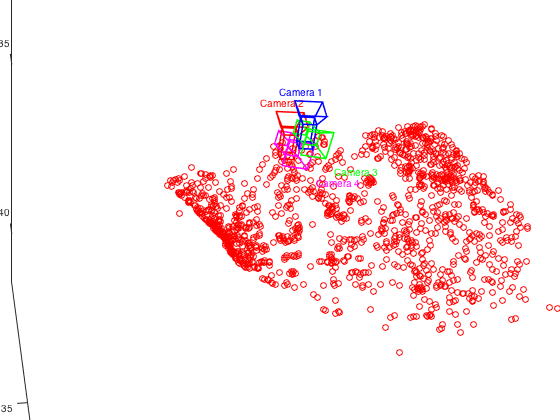
\includegraphics[width = \linewidth]{issues_with_triangulation2}

\end{document}
